\documentclass{article}
\usepackage[utf8]{inputenc}
\usepackage[T1]{fontenc}
\usepackage[frenchb]{babel}
\usepackage{graphicx}
\usepackage{color}
\usepackage{hyperref}
\usepackage{comment}
\newcommand{\shellcmd}[1]{\\\indent\indent\texttt{\footnotesize\# #1}\\}
\newcommand{\shellcmdd}[1]{\\\indent\indent\texttt{\footnotesize\# #1}}

\title{Manuel d'installation et d'utilisation de Google/CAPIRCA pour Telespazio (GCT)}
\author{Juan PIRON\\
   Elève ingénieur,\\
   4ème année \textit{Sécurité et Technologies Informatiques},\\
   {\color{red} Insa Centre Val de Loire},\\
   {\color{green} Campus de Bourges}\\
   \texttt{juan.piron@insa-cvl.fr}
}
\date{\today}

\begin{document}
  \maketitle

  \newpage
  \tableofcontents
  \newpage

  \section{Prérequis}

    Ce manuel n'a pas pour but de décrire l'architecture de Google/CAPIRCA.
    Ce manuel ne remplace d'aucune manière la documentation de Google/CAPIRCA, il apporte simplement les spécifités de GCT.
    Il est donc nécessaire de lire le README de Google/CAPIRCA.
    Pour cela il existe la \href{https://github.com/google/capirca/wiki}{wiki} GitHub de Google/CAPIRCA.
    \definecolor{orange}{RGB}{255,127,0}
    \colorbox{orange}{Toutes les adresses ips et les configurations présentes dans ce document sont fictives.}

  \section{Ce qu'est Google/CAPIRCA pour TPZ}

    Capirca est un outil conçu pour utiliser des définitions communes des réseaux, des services et des fichiers de règles (politiques) de haut niveau.
    Cela facilite le développement et la manipulation des listes de contrôle d'accès réseau (ACL) pour diverses plates-formes.
    CGT est Capirca appliqué à la gestion du PGL. Il permet de rendre plus rapide la prise en charge des demandes d'ouverture de flux utilisateur.
    \smallbreak

  \section{Ce que n'est pas Google/CAPIRCA pour TPZ}

    GCT ne remplace en aucun cas le manager (Cisco ASDM). C'est à dire que toutes modifications ou suppression d'une demande ce fait avec le manager.
    En d'autres termes pour supprimer une ACL ajouter à l'aide de CGT : \smallbreak
    1/ La supprimer dans le fichier .pol correspondant. \smallbreak
    2/ Aller sur le manager et la supprimer. \bigbreak
    \noindent Pour modifier : \smallbreak
    3/ réécrire le term correspondant à l'ACL dans le .pol. \smallbreak
    4/ recompiler \smallbreak
    Ne pas utiliser GCT pour une utilisation autre que celle décrite. Si le besoin et de créer des ACLs de type iptables,
    juniper ou encore cisco, veuillez utiliser le Google/CAPIRCA original.

  \section{Présentation du logiciel}

  Si vous détenez ce présent document c'est que vous avez aussi l'archive GCT.tar.gz. Cette archive contient 2 dossiers.
  Le premier contient les fichiers sources originaux de Google/CAPIRCA plus les dossiers sync et diff. \textit{sync/} et
  \textit{diff} contiennent les différents scripts d'adaptation de Capirca au PGL de TPZ. Sync s'occupe de la synchronisation
  des objets et diff d'éviter les doublons.
  A coter de \textit{capirca/} il y a gogsInstall qui contient tous le nécessaire pour l'installation.

  \section{Installation}

    Cette section concerne l'installation de Gogs sur le serveur (le manager) et le déploiement de GCT.
    L'installation décrite concerne un serveur Centos 7.

    \subsection{Prérequis}
      \subsubsection{MariaDB}

      Si la bdd n'existe pas alors l'installer :
\begin{verbatim}
      sudo yum -y update
      sudo yum -y install mariadb-server
      sudo service mariadb start
      mysql -u root -e "SET PASSWORD FOR 'root'@'localhost' = PASSWORD('password')
\end{verbatim}

      \subsubsection{Python}

      Version 2.7 ou supérieur. \bigbreak
      \noindent Installer pip :
      \noindent\shellcmdd{curl \"https://bootstrap.pypa.io/get-pip.py\" -o \"get-pip.py\"}
      \noindent\shellcmdd{python get-pip.py} \smallbreak
      \noindent Installer paramiko :
      \noindent\shellcmdd{yum install gcc libffi-devel python-devel openssl-devel}
      \noindent\shellcmdd{pip install cryptography}
      \noindent\shellcmdd{pip install paramiko} \smallbreak
      \noindent Installer netmiko :
      \noindent\shellcmdd{pip install scp}
      \noindent\shellcmdd{pip install pyyaml}
      \noindent\shellcmdd{pip install pytest}

    \subsubsection{SSH}

      Avoir openssh-server sur le serveur et configuré ssh avec un utilisateur ssh "git" sur le PGL. \bigbreak
      \noindent Firewall PGL : \smallbreak
\begin{verbatim}
      hostname(config)# crypto key generate rsa modulus 1024
      hostname(config)# write memory
      hostanme(config# aaa authentication ssh console LOCAL
      hostanme(config# username git password password
      hostname(config)# ssh timeout 30
      hostname(config)# ssh version 2
\end{verbatim}
      Cette example de configuration a été fait à partir de une maquette qui utilise un cisco ASA 5520.
      Il peut donc y avoir des différences avec le PGL. Eviter d'utiliser les certificats, sinon modifier les scripts
      pre-receive et post-receive.
      \noindent Entre le client et gogs-server : \bigbreak
      Sur un client :
      \shellcmdd{ssh-keygen -t rsa}
      \shellcmdd{chmod 700 ~/.ssh}
      \shellcmdd{chmod 600 ~/.ssh/id\_rsa}
      \shellcmdd{chmod 644 ~/.ssh/id\_rsa.pub}
      \shellcmdd{chmod  ~/.ssh/know\_hosts} \smallbreak
      Envoyer la clé public id\_rsa.pub public du poste client au server. \bigbreak
      Sur le serveur :
      \shellcmdd{cat id\_rsa.pub >> ~/.ssh/authorized\_keys}
      \shellcmdd{chmod 700 ~/.ssh}
      \shellcmdd{chmod 644 ~/.ssh/authorized\_keys}
      \shellcmdd{chmod 600 ~/.ssh/id\_rsa}
      \shellcmdd{chmod 644 ~/.ssh/id\_rsa.pub} \smallbreak

      \noindent Dans /etc/ssh/sshd\_config désactiver PasswordAuthentication et ainsi forcer l'utilisation des clés :
\begin{verbatim}
      PasswordAuthentication no
\end{verbatim}

    \subsubsection{Autres}

      Configurer SELinux de manière à permettre l'accès à ssh (scp) au dossier tmp pour l'échange des clés.
      \noindent Installer Git : \shellcmdd{yum -y install git} \smallbreak
      \noindent Une fois Capirca importé il faut installer les prérequis dans \textit{capirca/} à l'aide de :
      \shellcmdd{pip install -r requirements.txt}

    \subsection{Procédure}

      Sur le serveur "manager" créer l'utilisateur git et définir son mot de passe : \shellcmd{useradd -m git}
      Ajouter pour l'installation, git au groupe sudo : \shellcmd{usermod -aG wheel git}
      Ne pas oublier de l'en retirer après l'installation. \smallbreak
      \noindent Décompresser gogsInstall.tar.gz dans \textit{/home/git} : \shellcmd{tar -xzvf gogsInstall.tar.gz}
      Ce déplacer dans le dossier gogsInstall éditer les scripts python pre-receive et post-receive.
      L'adresse ip qui doit être rentrer et celle du PGL, de même que le couple id/password ssh :
\begin{verbatim}
      pgl = {
        'device_type':'cisco_asa',
        'ip':'192.168.1.1',
        'username':'intern',
        'password':'tpzinsacvl',
        'secret':'tpzinsacvl',
      }
\end{verbatim}
      Editer app.ini, faire correspondre l'adresse ip et le domain avec ceux du serveur :
\begin{verbatim}
      [server]
      PROTOCOL = http
      DOMAIN = 192.168.1.10
      ROOT_URL = %(PROTOCOL)s://%(DOMAIN)s:%(HTTP_PORT)s/
      HTTP_ADDR = 192.168.1.10
\end{verbatim}
      Ajouter les droits d'execution au script gogsInstall.sh : \shellcmd{chmod u+x gogsInstall.sh}
      Exécuter le script en scpécifiant le mot de passe root de mariadb comme arg1. Scpéfier le mot de passe que vous voulez donner
      à l'utilisateur git de mariadb en arg2 : \shellcmd{./gogsInstall.sh mdp-root-mariadb mdp-git-mariadb}
      Ouvrir un navigateur et rentrer l'url : \url{http://ip-du-serveur:3000} \smallbreak
      \noindent Une page d'installation s'ouvre, il suffit d'entrer le mot de passe de l'utilisateur git de la bdd mariadb et de confirmer.

    \subsection{Déploiement}

      Pour l'utilisation de Gogs se référer à sa \href{https://gogs.io/docs}{documentation}. \bigbreak
      \noindent Créer un utilisateur "tpz". A l'aide de tpz ajouter un repository distant nommer "GCT".
      Décompresser GCT.tar.gz, uploader capirca dans GCT. Créer d'autres utilisateurs et les incorporer comme participant en "rw".
      Récupérer les différentes clés ssh des postes qui cloneront GCT et les ajouter à tpz en allant dans ses paramètres.
      Ne pas les ajouter au repository mais bien directement dans les paramètres de l'utilisateur tpz.
      Enfin récuperer la wiki dans \textit{CGT/} et l'ajouter au repository GCT.
\begin{comment}
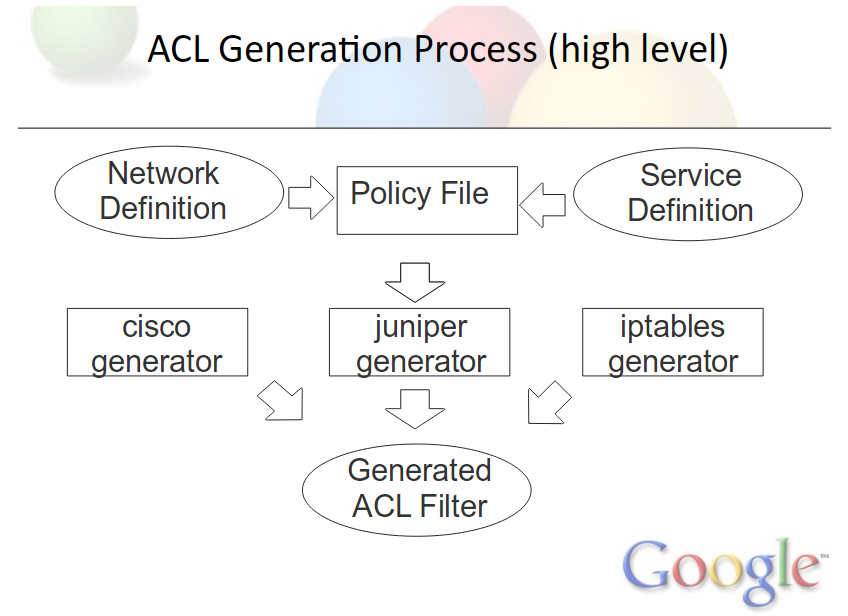
\includegraphics[scale=0.4]{capirca.png}
\end{comment}

  \section{Utilisation}
    \subsection{Configuration du dépôt local et du client}

      Avant tout transférer sa clé rsa (ssh) à l'admin. Ensuite se placer dans un nouveau repertoire et faire un \texttt{git init}.
      L'étape suivante et de configurer localement Git à l'aide de : \shellcmdd{git config --global user.name "John Doe"}
      \shellcmdd{git config --global user.email johndoe@example.com}\smallbreak
      \noindent Le nom spécifié sera celui qui apparaîtra sur les commits.
      Pour une demande d'ouverture de flux utilisateur créer autant de fichier .pol qu'il y a d'interfaces du PGL concernées.
      Dans le header le champ \texttt{target::} doit avoir pour nom celui de l'interface.
      Capirca ne comprend que les objets, que cela soit pour les réseaux ou les services.
      Avant de créer un .pol il faut donc créer les objets. Pour les réseaux les ajouter en début du fichier \textit{capirca/def/NETWORK.net}
      et pour les services dans \textit{capirca/def/SERVICES.svc}. GCT récupère de manière automatique les objets présent
      sur le PGL, donc regarder d'abord si l'objet existe en faisant un CTRL-F en spécifiant de l'ip ou du service.
      Les demandes au format .pol doivent se trouver dans le dossier \textit{capirca/policies/pol}.
      Après avoir terminer de créer les différents fichier .pol, dans \textit{capirca/} lancer le script  : \texttt{./run.sh} \smallbreak
      \noindent Quand on vous le demandera, entrer un commit. Tous les commits doivent être de la forme : \texttt{ajout de ref-de-la-demande} ou
      \texttt{modification de ref-de-la-demande}. Pour une suppresion ou modification faire comme indiqué dans \textit{Ce que n'est pas GCT}.
      \bigbreak Récapitulation : \smallbreak
      1/ Rechercher ou créer les objets \smallbreak
      2/ Créer les .pol \smallbreak
      3/ \texttt{./run.sh} \bigbreak
      \noindent Si lors de la compilation (abus de langage) il se produit un Git "CONFLICT" se référer à la partie \textit{Rappel succint
      sur les commandes Git}.
      Avant tout essai assurez-vous d'avoir bien toutes les librairies python requises d'installées : \smallbreak
      - gflags (\texttt{pip install python-gflags}) \smallbreak
      - getopt \smallbreak
      - csv \smallbreak
      - re (\texttt{pip install regex}\smallbreak
      - socket \smallbreak
      - netaddr

    \subsection{Exemple}

      Voici un exemple de configuration d'une demande .pol et des objets. \smallbreak
\begin{verbatim}
      ------ .POL -------

      header {
        comment:: "Demandeur : Tintin"
        comment:: "Realisee par : Cpt. Hadock"

        target:: ciscoasa Eth1_CSG
      }

      term NTP {
        source-address:: REMUS1
        protocol:: udp
        source-port:: NTP_SOURCE
        destination-address:: REMUS2
        destination-port:: NTP_DEST
        logging:: syslog
        action:: accept
      }

      term SYSLOG {
        source-address:: A_192_168_1_2
        protocol:: udp
        source-port:: SYSLOG_SOURCE
        destination-address:: SSI
        destination-port:: SYSLOG_DEST
        logging:: syslog
        action:: accept
      }

      ------ NETWORK.net -------

      REMUS1 = 192.168.10.0/24
      REMUS2 = 192.168.20.0/24
      REMUS10 = 192.168.100.0/24
      REMUS11 = 192.168.110.0/24
      A_192_168_1_2 = 192.168.1.2/32
      SSI = 192.168.30.0/24

      ------ SERVICES.svc -------

      NTP_SOURCE = 123/udp
      NTP_DEST = 123/udp
      SYSLOG_SOURCE = 514/udp
      SYSLOG_DEST = 1024-65535/udp
      Netbios-src = 135/tcp
                    139/tcp
      Netbios-dest = 1024-65535/tcp
\end{verbatim}

    \subsection{Recommandations}

      Ne pas utiliser de charactères spéciaux.
      Ne pas utiliser de : \ ou d'accents.
      Ne pas écrire de \texttt{remark:: } trop longue, la limite est de 50 charactères.


  \section{Rappels succincts sur les commandes Git}

    En cas de conflit Git c'est toujours mieux de se souvenir des commandes importantes. \bigbreak
    \noindent\texttt{git init} : initialise un repertoire vide \smallbreak
    \noindent\texttt{git clone https://...} : récupère un projet (correspond à un fetch + un merge) \bigbreak
    \noindent En local : \bigbreak
    \noindent\texttt{git add fichier.txt} \smallbreak
    \noindent\texttt{git add -A } : tous \smallbreak
    \noindent\texttt{git commit fichier.txt -m blablabla ou git commit -a blabla} \smallbreak
    \noindent\texttt{git commit --amend} : modifier le dernier commit (ex : faute de frappe). \bigbreak
    \noindent Travail avec un depôt distant : \bigbreak
    \noindent\texttt{git remote add origin https://...} : ajout d'un depôt distant, origin correspond au nom que l'on donne au dépôt \smallbreak
    \noindent\texttt{git remote -v} : liste les reps distants (dépôts) \smallbreak
    \noindent\texttt{git remote rm origin} : supprime le remote origin \smallbreak
    \noindent\texttt{git pull origin master} : mise à jour avec la branche master du dépôt origin \smallbreak
    \noindent\texttt{git push origin master} : on envoie à la branche master du dépôt origin nos modifs \bigbreak
    \noindent Les branches : \bigbreak
    \noindent\texttt{git branch test} : créer une branche test en local \smallbreak
    \noindent\texttt{git branch} : liste les branches présentes \smallbreak
    \noindent\texttt{git push orgin test} : permet de pusher sur la nouvelle branche mais aussi de la créer sur le dépôt distant \smallbreak
    \noindent\texttt{git checkout test} : permet de switcher entre les différentes branches \smallbreak
    \noindent\texttt{git merge test} : depuis la branche master, permet de fusionner le travail de la branche test \smallbreak
    \noindent\texttt{git push origin --delete test} : supprime la branche dans le rep distant \smallbreak
    \noindent\texttt{git branch -d test} : supprime la branche localement \bigbreak
    \noindent Le stash : \bigbreak
    \noindent\texttt{git stash} : pour mettre de côté un travail que l'on ne veut pas commit si on doit changer de branch \smallbreak
    \noindent\texttt{git stash apply ou git stash apply stash@\{0\}} : pour le récupérer au retour \smallbreak
    \noindent\texttt{git stash list} : affiche la pile \smallbreak
    \noindent\texttt{git stash drop stash@\{0\}} : supprime le stash \smallbreak
    \noindent\texttt{git stash pop} : pour appliquer la remise puis la suprimer \bigbreak
    \noindent Les différences : \bigbreak
    \noindent\texttt{diff master origin/master} : différence entre la branche local et celle dans le rep distant \bigbreak
    \noindent Revenir en arriere : \bigbreak
    \noindent\texttt{git log} : lister les commits ( et voir le num) \smallbreak
    \noindent\texttt{git checkout <commit>} : revenir au commit indiqué comme spectateur \smallbreak
    \noindent\texttt{git reset --hard} : revenir au dernier commit \smallbreak
    \noindent\texttt{git reset <commit> --hard} : revenir au commit indiqué \bigbreak
    \noindent Les différentes copies dans gits : \bigbreak
    \noindent workspace, index, local repository, remote repository \bigbreak
    \noindent add : workspace --> index \smallbreak
    \noindent commit : index --> local \smallbreak
    \noindent push : local --> remote \smallbreak
    \noindent fetch : remote --> local \smallbreak
    \noindent merge : local --> workspace \smallbreak
    \noindent pull : remote --> workspace

\end{document}
